\section{The Implementation}

The parallel implementation lies within {\tt parallel.c}. Most of this should be
relatively straightforward for people with basic knowledge in OpenMP and MPI,
but a small description of the changes from the original program will be given.

For single for loops, the single loop is prepended with a pragma, and an
eventual {\tt omp\_id} is defined inside. The id is used whenever multiple {\tt
  z} buffers are needed, and we don't want to allocate and free buffers if we
can avoid so. Henceforth, we make an array of buffers, and as such, {\tt z} is
a {\tt Real**} instead. The listing below is an example of such a setup.

\begin{lstlisting}
#pragma omp parallel for private(omp_id)
for (i=0; i < mpi_work; i++) {
  omp_id = omp_get_thread_num();
  fst_(b[j], &n, z[omp_id], &nn);
}
\end{lstlisting}

For double for loops, we only ensure that the inner loop's iterator is private,
and add this variable inside the private declaration in the OpenMP pragma.

As for the OpenMP reduction, we perform a local reduction through a specialized
OpenMp implementation, and send the result of the local reduction to a global
MPI reduction. The result is stored within the node with rank 0, and is printed
out afterwards.

\subsection{Transpose}

Instead of using \verb|MPI_Alltoallv|, we ended up using \verb|MPI_Alltoall|.
This requires repetitive calls to {\tt Alltoall}, so at first one may assume
that this may be slower than using {\tt Alltoallv}. However, the speed may be
roughly the same, and it may not be unrealistic that {\tt Alltoall} is faster
than {\tt Alltoallv}. This is because {\tt Alltoall} is easier for MPI to
optimize, whereas it is outright hard to optimize {\tt Alltoallv} as it has a
vast amount of configuration possibilities.

\begin{figure}[h]
  \centering
  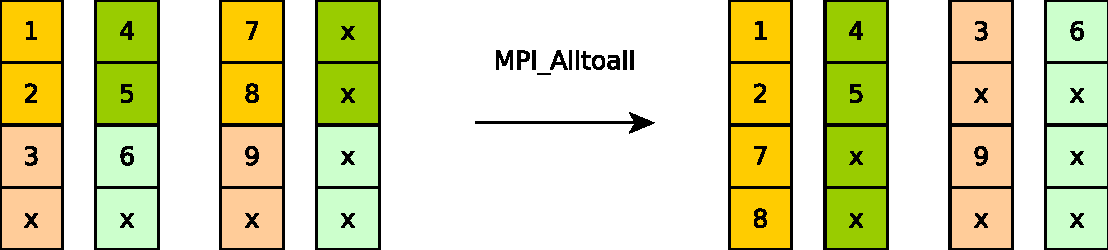
\includegraphics[width=0.8\textwidth]{img/transpose-1.pdf}
  \caption{The result of performing {\tt MPI\_Alltoallv} in the implementation.}
  \label{fig:t1}
\end{figure}

We then perform a local transponation. This works as follows: We perform a local
transponation on each square block we store in memory. The square block's size
has the amount of rows each node contains multiplied with the amount of nodes.
Consequently, each row may be a bit larger than the original $m$, with the
result of a simpler transpose implementation which may be potentially faster
than using {\tt Alltoallv}.

\begin{figure}[h]
  \centering
  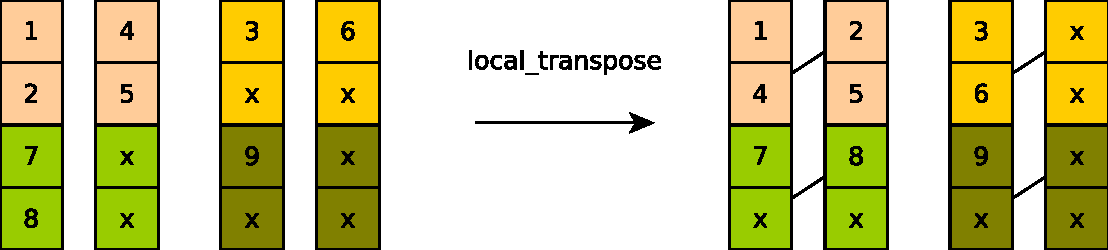
\includegraphics[width=0.8\textwidth]{img/transpose-2.pdf}
  \caption{Performing {\tt local\_transpose} in the implementation.}
  \label{fig:t2}
\end{figure}

In order to load balance as much as possible, the last node will potentially do
less work than the other nodes, compared to the other scenario where it has to
perform more work. Both Figure \ref{fig:t1} and \ref{fig:t2} shows the edge case
where the last node has not as many rows to work with as the previous nodes.
